%===============================================================================
% Project description
%===============================================================================
% $Id$
%===============================================================================


%===============================================================================
% Configuration
%===============================================================================


%-------------------------------------------------------------------------------
% \documentclass and \usepackage directives
%-------------------------------------------------------------------------------
\documentclass[a4paper,fleqn,titlepage]{article} 
%\usepackage{ngerman}
\usepackage[latin1]{inputenc}
\usepackage[T1]{fontenc}
\usepackage[small,hang,bf]{caption2}
\usepackage{fancyhdr}
\usepackage[nice]{nicefrac}
\usepackage{color,listings}
\usepackage{alltt}


% Compilation with latex or pdflatex?
\newif\ifpdf 
\ifx\pdfoutput\undefined 
  \pdffalse
\else
  \pdfoutput=1 
  \pdftrue 
\fi 

% Compilation with pdflatex
\ifpdf
 
  \usepackage[pdftex]{graphicx}

  \usepackage[
    pdftex,
    a4paper,
    bookmarks,
    pdfstartview=FitH,    % starts with page width
    bookmarksopen,        % opens index
    bookmarksnumbered,    % index with numbering
    colorlinks,           % links with color, otherwise with border
    linkcolor=blue,       % Standard red
    citecolor=blue,       % Standard green
    urlcolor=magenta,     % Standard cyan
    filecolor=blue
  ]{hyperref} 

  \pdfinfo{
    /Title      (Project description)
    /Author     (Thomas Weibel, Martin Luder, Michael K�ser)
    /Subject    (Eiffel programming)
    /Keywords   (Programming, EiffelRSS)
  }

  % Use default Acrobat reader fonts
  \usepackage{mathpazo}

  % Use CM fonts (increases document size)
  % \usepackage{ae}

% Compilation with latex
\else 

  \usepackage{graphicx} 

\fi


%-------------------------------------------------------------------------------
% Configure \maketitle
%-------------------------------------------------------------------------------
\title{EiffelRSS \\ Project description}
\author{
  Michael K\"aser <kaeserm@student.ethz.ch>
  \and 
  Martin Luder <luderm@student.ethz.ch>
  \and 
  Thomas Weibel <weibelt@student.ethz.ch>
}
\date{\today}


%-------------------------------------------------------------------------------
% Configure fancyhdr
%-------------------------------------------------------------------------------
\pagestyle{fancy}

\renewcommand{\headrulewidth}{0.1 pt}
\renewcommand{\footrulewidth}{0.1 pt}

\fancypagestyle{plain}{
  \lhead{\nouppercase{\leftmark}}
  \chead{}
  \rhead{\thepage}
  \lfoot{EiffelRSS}
  \cfoot{}
  \rfoot{Project description}
}

\lhead{\nouppercase{\leftmark}}
\chead{}
\rhead{\thepage}

\lfoot{EiffelRSS}
\cfoot{}
\rfoot{Project description}


%-------------------------------------------------------------------------------
% Configure listings
%-------------------------------------------------------------------------------
\lstset{showstringspaces=false,
  breaklines=true,
  breakindent=0pt,
  prebreak=\mbox{\tiny$\searrow$},
  postbreak=\mbox{{\color{blue}\tiny$\rightarrow$}},
  frame=trBL,
  framerule=0.75pt,
  framesep=4pt,
  rulesep=0.75pt
}


%-------------------------------------------------------------------------------
% Common configuration
%-------------------------------------------------------------------------------
\setlength{\parindent}{0em}
\setlength{\parskip}{1.5ex plus0.5ex minus0.5ex}
\sloppy
\setlength{\mathindent}{0em}


%-------------------------------------------------------------------------------
% Commandos
%-------------------------------------------------------------------------------
\newcommand{\hr}{\rule{\textwidth}{1pt}}


%===============================================================================
% Document
%===============================================================================
\begin{document}

\begin{titlepage}
  \newlength{\centeroffset}
  \setlength{\centeroffset}{-0.5\oddsidemargin}
  \addtolength{\centeroffset}{0.5\evensidemargin}

  \thispagestyle{empty}

  \noindent
\includegraphics[width=\textwidth]{../figures/big_ETH}\\[-3mm]
  \hr

  \vspace*{\stretch{1}}

  \makebox[0pt][l]{
    \begin{minipage}{\textwidth}
      \flushright{
        \Huge\bfseries EiffelRSS
      }

      \noindent\rule{\textwidth}{3pt}\\[2.5ex]

      \hfill\emph{
        \Large Project description
      }
    \end{minipage}
  }

  \vspace{\stretch{1}}

  \makebox[0pt][l]{
    \begin{minipage}{\textwidth}
      \flushright{
        \bfseries 
        Michael K\"aser <kaeserm@student.ethz.ch>\\[0.3ex]
        Martin Luder <luderm@student.ethz.ch>\\[0.3ex]
        Thomas Weibel <weibelt@student.ethz.ch>\\[0.3ex]
      }
    \end{minipage}
  }

  \vspace{\stretch{1}}

  \noindent\hr\\[1mm]
  
\includegraphics[width=\textwidth]{../figures/big_inf}
\end{titlepage}

\begin{abstract}
  EiffelRSS is an Eiffel library to parse RSS. The goal is to provide
  the Eiffel development community with an easy to use and well
  structured API for RSS.
  
  The distribution also contains a RSS newsfeed reader written with
  EiffelVision and EiffelRSS.
\end{abstract}


\section{Library}
\label{sec:overview}

The library of EiffelRSS consists of several different clusters.


\subsection{ADT}
\label{sec:adt}

\texttt{ADT} contains the deferred classes \texttt{SORTABLE} and
\texttt{ORDER\_RELATION} which can be used to implement sortable
structures. 

\texttt{SORTABLE\_TWO\_WAY\_LIST} inherits from \texttt{SORTABLE} and
\texttt{TWO\_WAY\_LINKED\_LIST} to implement a sortable doubly-linked
list.

See figure \ref{fig:adt} for an overview of the cluster.

\begin{figure}[htbp]
  \centering
  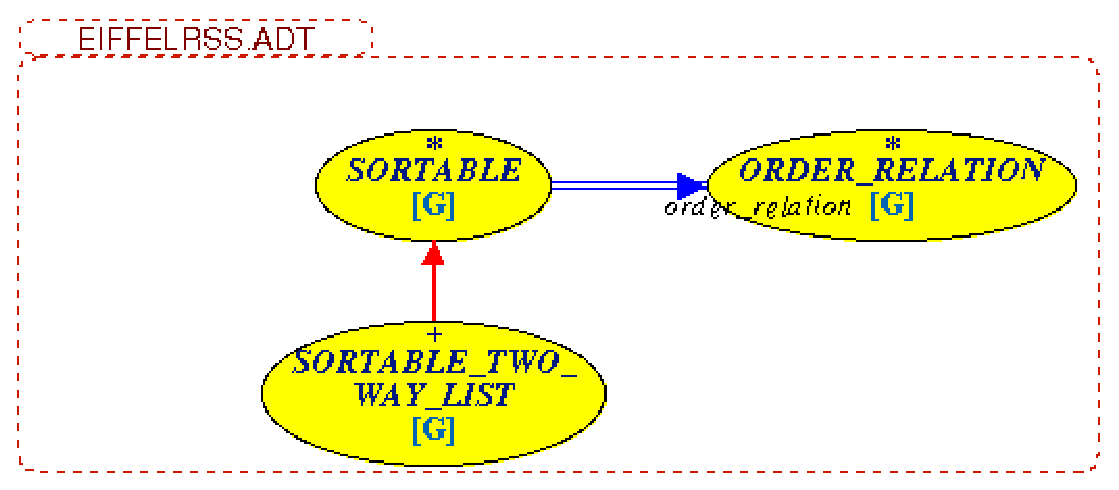
\includegraphics[width=0.7\textwidth]{./figures/EIFFELRSS_ADT}
  \caption{BON diagram of cluster \texttt{ADT}}
  \label{fig:adt}
\end{figure}


\subsection{FETCH}
\label{sec:fetch}

\texttt{FETCH} is a class which has features that can fetch data from
a source address to a local \texttt{STRING} using various services.
\texttt{FETCH} provides a simple interface for the
\texttt{DATA\_RESOURCE} class in EiffelNet.

A valid source address has the following format:
\texttt{service://address}.

Supported services are: file, http, ftp.

See figure \ref{fig:fetch} for an overview of the cluster.

\begin{figure}[htbp]
  \centering
  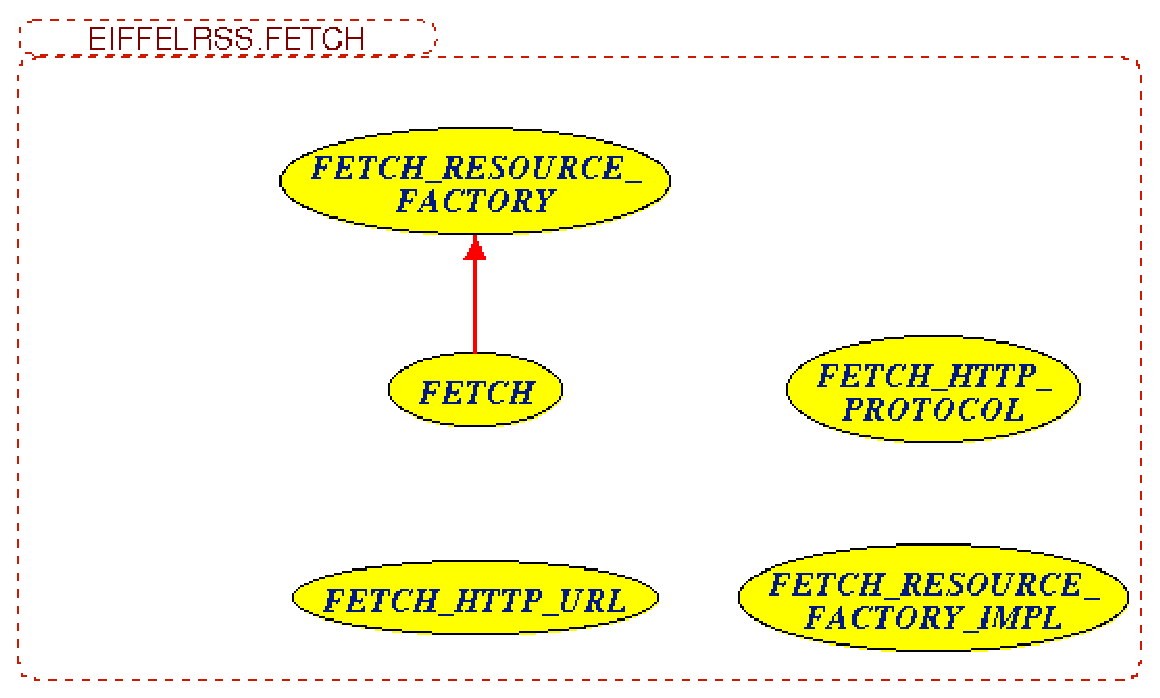
\includegraphics[width=0.7\textwidth]{./figures/EIFFELRSS_FETCH}
  \caption{BON diagram of cluster \texttt{FETCH}}
  \label{fig:fetch}
\end{figure}


\subsection{LOGFILE}
\label{sec:logfile}

\texttt{LOGFILE} represents a file which can be used for logging
messages during the program execution.

Each message has its own priority (a positive integer value) and each
logfile a certain user defined threshold. If the priority of the
message is greater or equal than the threshold, it gets written to the
log file together with a timestamp.

See figure \ref{fig:logfile} for an overview of the class.

\begin{figure}[htbp]
  \centering
  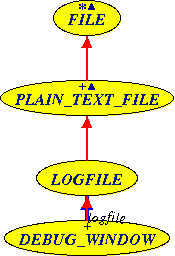
\includegraphics[scale=.6]{./figures/LOGFILE}
  \caption{BON diagram of class \texttt{LOGFILE}}
  \label{fig:logfile}
\end{figure}


\subsection{PROPERTIES}
\label{sec:properties}

\texttt{PROPERTIES} represents a persistent set of properties. The
properties can be saved to a file or loaded from a file.

Each key and its corresponding value in the property list is a string.

A property list can contain another property list as its default. This
default property list is searched if the property key is not found in
the original property list.

\texttt{PROPERTIES} is similar to the \texttt{java.util.Properties}
class. The main difference is, that \texttt{PROPERTIES} doesn't
support keys and values separated by whitespace only. It always
expects \texttt{:} or \texttt{=} as a separator between key and value.

See figure \ref{fig:properties} for an overview of the cluster.

\begin{figure}[htbp]
  \centering
  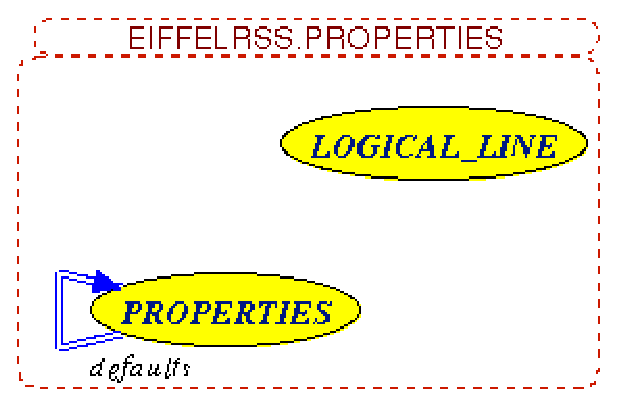
\includegraphics[scale=.6]{./figures/EIFFELRSS_PROPERTIES}
  \caption{BON diagram of cluster \texttt{PROPERTIES}}
  \label{fig:properties}
\end{figure}


\subsection{SYNDICATION}
\label{sec:syndication}

\texttt{SYNDICATION} is the main cluster of EiffelRSS with a feed
object model, and classes to load and write feeds. It is divided into
three subclusters.

See figure \ref{fig:syndication} for an overview of the cluster.

\begin{figure}[htbp]
  \centering
  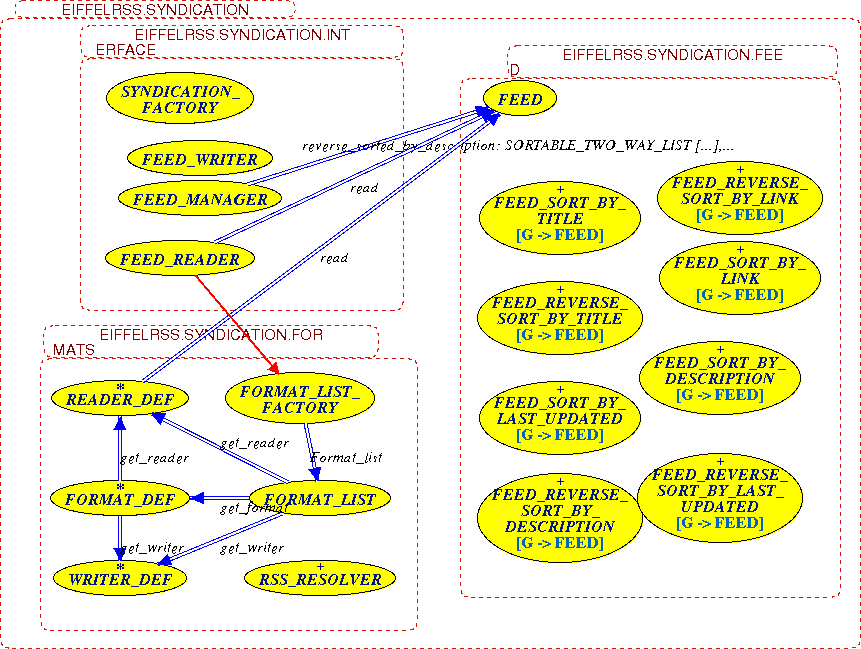
\includegraphics[width=\textwidth]{./figures/EIFFELRSS_SYNDICATION}
  \caption{BON diagram of cluster \texttt{SYNDICATION}}
  \label{fig:syndication}
\end{figure}


\subsubsection{INTERFACE}

\texttt{INTERFACE} is the sub-cluster of syndication with all the
classes a developer needs to use the library. There are classes to
read into and write from a \texttt{FEED}, a \texttt{FEED\_MANAGER} to
administrate a list of \texttt{FEED}s, and a factory class which makes
it easy to create all necessary objects.

See figure \ref{fig:interface} for an overview of the cluster.

\begin{figure}[htbp]
  \centering
  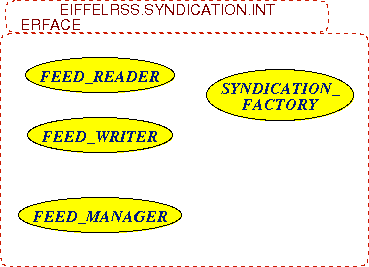
\includegraphics[scale=.6]{./figures/EIFFELRSS_SYNDICATION_INTERFACE}
  \caption{BON diagram of cluster \texttt{INTERFACE}}
  \label{fig:interface}
\end{figure}


\subsubsection{FEED}

\texttt{FEED} is the central datastructure of EiffelRSS. t defines an
abstract syndication feed.

See figure \ref{fig:feed} for an overview of the cluster.

\begin{figure}[htbp]
  \centering
  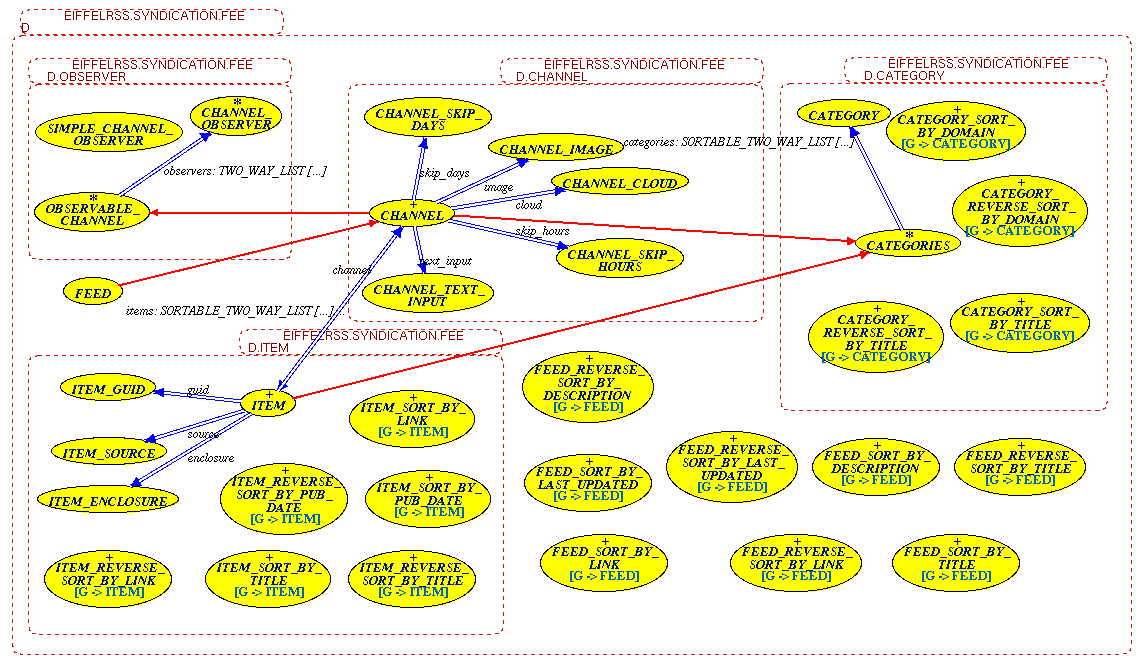
\includegraphics[width=\textwidth]{./figures/EIFFELRSS_SYNDICATION_FEED}
  \caption{BON diagram of cluster \texttt{FEED}}
  \label{fig:feed}
\end{figure}


\subsubsection{FORMATS}

\texttt{FORMATS} defines the different syndication formats.

See figure \ref{fig:formats} for an overview of the cluster.

\begin{figure}[htbp]
  \centering
  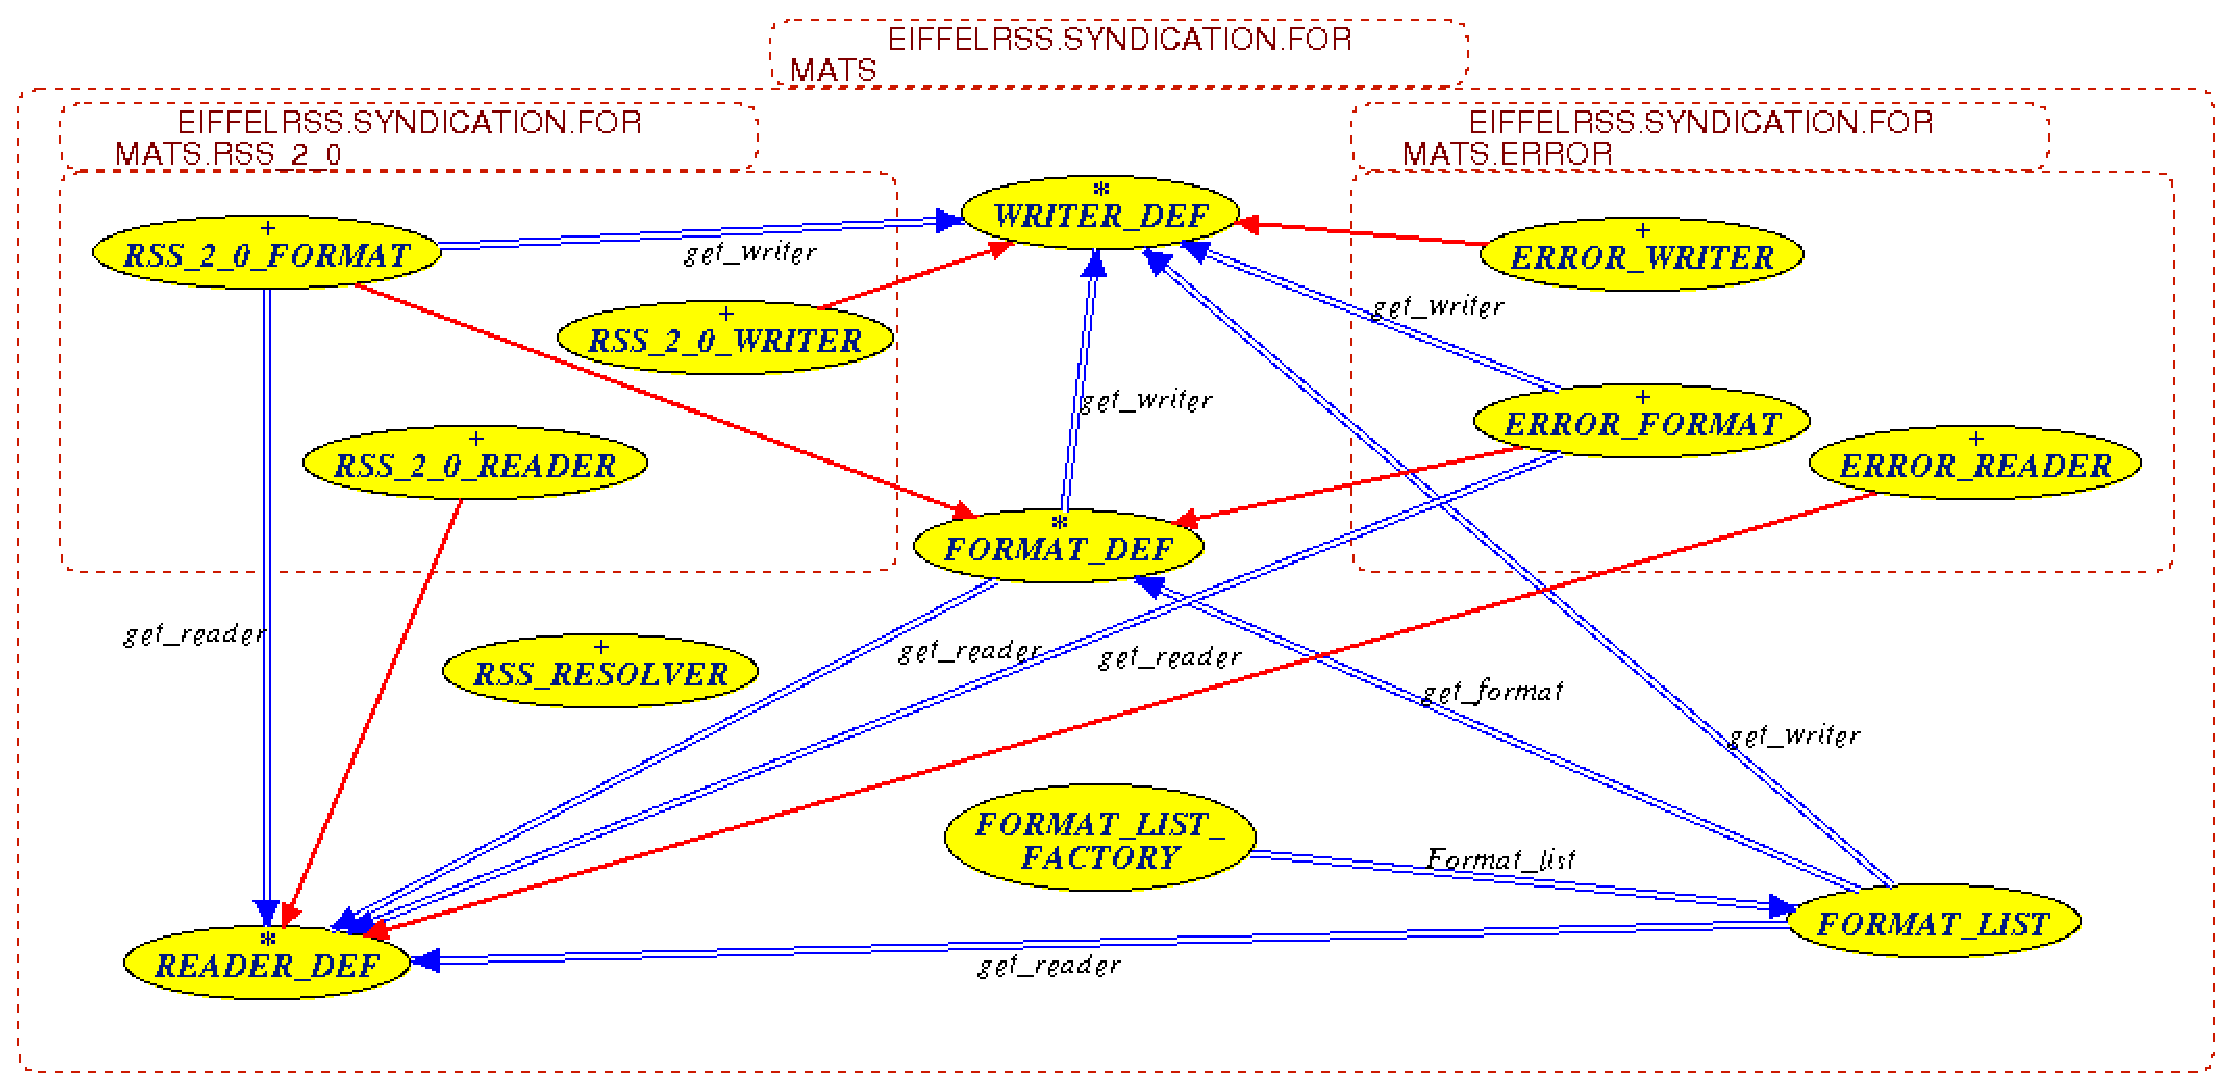
\includegraphics[width=\textwidth]{./figures/EIFFELRSS_SYNDICATION_FORMATS}
  \caption{BON diagram of cluster \texttt{FORMATS}}
  \label{fig:formats}
\end{figure}


\section{Newsreader}
\label{sec:newsreader}

Newsreader is a simple GUI, with which you can read your RSS feeds. In
addition to the GUI it also has a command line user interface.

It is possible to add custom feeds and open news in your Internet
browser.

Figure \ref{fig:newsreader} shows a screenshot of the graphical user
interface.

\begin{figure}[htbp]
  \centering
  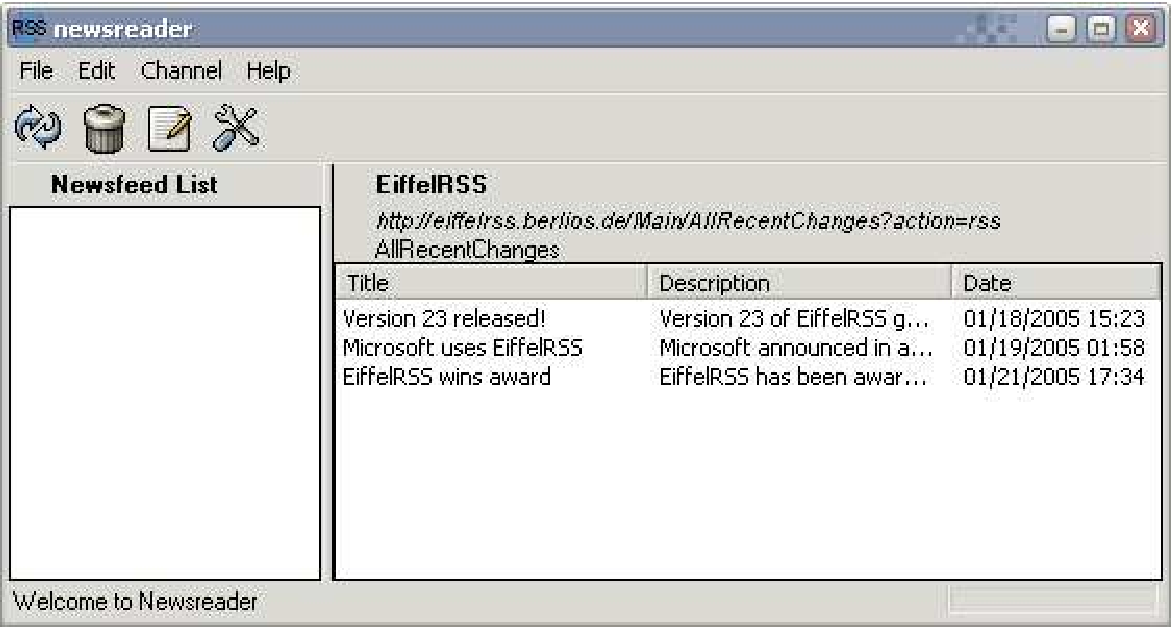
\includegraphics[width=0.7\textwidth]{./figures/newsreader}
  \caption{Screenshot of the graphical user interface of Newsreader}
  \label{fig:newsreader}
\end{figure}


\section{Extensibility}
\label{sec:extensibility}

EiffelRSS is designed with extensibility in mind.

Initially EiffelRSS will only support reading of RSS 2.0. But the
library is designed to be easily extensible by other RSS readers. Even
non-RSS syndication formats like Atom can be parsed into EiffelRSS'
datamodel. It is also feasible to add writing support and to write any
syndication format (even non-XML). Because EiffelRSS uses an abstract
intermediate representation of newsfeed data, one can also convert
from one format to another.

Another possibility of extension would be the newsfeed reader written
with EiffelVision. This application could be extended to a full
fledged newsfeed reader.


\section{Who does what?}
\label{sec:who_does_what}


\subsection{All project members}
\label{sec:all}

\begin{itemize}
\item Writing documentation
\item Testing
\end{itemize}


\subsection{Michael K�ser}
\label{sec:michael}

\begin{itemize}
\item The clusters \texttt{LOGFILE} and \texttt{FETCH}
\item An abstraction for readers and writers which translate between
  XML files and the \texttt{FEED} object structure
\item An implementation of RSS 2.0
\end{itemize}


\subsection{Martin Luder}
\label{sec:martin}

\begin{itemize}
\item Newsreader with graphical and command line user interface
\end{itemize}


\subsection{Thomas Weibel}
\label{sec:thomas}

\begin{itemize}
\item The clusters \texttt{ADT} and \texttt{PROPERTIES}
\item \texttt{FEED} data model
\end{itemize}

\end{document}
